% This is samplepaper.tex, a sample chapter demonstrating the
% LLNCS macro package for Springer Computer Science proceedings;
% Version 2.20 of 2017/10/04
%
\documentclass[runningheads]{llncs}
%
\usepackage{graphicx}
\usepackage{verbatim}
% Used for displaying a sample figure. If possible, figure files should
% be included in EPS format.
%
% If you use the hyperref package, please uncomment the following line
% to display URLs in blue roman font according to Springer's eBook style:
% \renewcommand\UrlFont{\color{blue}\rmfamily}
\usepackage{url}
\begin{document}
%
\title{Towards a Formally Verified EVM in Production Environment}
%
%\titlerunning{Abbreviated paper title}
% If the paper title is too long for the running head, you can set
% an abbreviated paper title here
%
\author{Xiyue Zhang\inst{1} \and
Yi Li\inst{1} \and
Meng Sun\inst{1}
}
%
% \authorrunning{F. Author et al.}
% First names are abbreviated in the running head.
% If there are more than two authors, 'et al.' is used.
%
\institute{School of Mathematical Sciences, Peking University
\\
\email{\{xiyuezhang, liyi\_math, sunm\}@pku.edu.cn}}
%
\maketitle              % typeset the header of the contribution
%
\begin{abstract}
Among dozens of decentralized computing platforms, Ethe\-reum attracts widespread attention for its native support of smart contracts by means of a virtual machine called EVM. Programs can be developed in various front-end languages. For example, Solidity can be deployed to the blockchain in the form of compiled EVM opcodes. However, such flexibility leads to critical safety challenges. In this paper, we formally define the behavior of EVM in Why3, a platform for deductive program verification, which facilitates the verification of different properties. Furthermore, the extracted implementation in OCaml can be directly integrated into the production environment and tested against the standard test suite. The combination of proofs and testing in our framework serves as a powerful analysis basis for EVM and smart contracts.

\keywords{EVM \and Why3 \and Verification \and Testing.}
\end{abstract}
%
%
%
\section{Introduction}
Ever since the inception of the Bitcoin \cite{nakamoto2008bitcoin} blockchain system, cryptocurrencies have become a global revolutionary phenomenon known to majority of people. Meanwhile, the decentralized system with no server or central authority, which emerges as a side product of Bitcoin, shows great potential in carrying out secure online transactions. From then until now, there have been so much change and growth on blockchain technology. The researchers and developers see plenty of potential and massive possibilities of blockchain applications, especially in financial, governmental services. Ethereum\cite{Ethereum} extends Bitcoin's design, which can not only process transactions but also process complex smart contracts and programs. This feature makes Ethereum a popular ecosystems for building blockchain-applications, which gains much more interest to innovate the options to utilize blockchain.

Smart contracts are often written in a high level programming language called \textit{Solidity} \cite{solidity} and then compiled into low-level machine instructions (\textit{opcodes}), which is encoded into bytecode. Ethereum Virtual Machine (EVM) is a quasi-Turing complete machine which implements the execution model of the Ethereum. Given a sequence of bytecode instructions, which are compiled from smart contracts by EVM compiler, and the environment data, this execution model specifies how the blockchain transits from one state to another. 

However, EVM and smart contracts are faced with several security vulnerabilities. Atzei et al. presented a taxonomy of vulnerabilities and related attacks against Solidity, the EVM, and the blockchain in \cite{atzei2016survey}. The adoption of formal methods can facilitate the production of trustworthy and reliable software systems. Verification such as theorem proving techniques and testing have become essential to guarantee the correctness of safety-critical systems. 

To address the security challenges against EVM, we present a framework of generating formally verified EVM for production environment in this paper. The contributions of this work are: Firstly, a formal definition of EVM is specified in WhyML, the language of programming and specification in Why3. Secondly, an implementation of EVM in OCaml is generated through an extraction mechanism based on a series of customized drivers. Lastly, the verification of sample properties and testing of the OCaml implementation for EVM against a standard test suite for Ethereum.

This paper is organized as follows: Section \ref{Sec: Pre} presents some background about Why3, Ethereum Virtual Machine (EVM) and smart contracts. We outline the framework for formalizing, property verifying and testing of EVM in Section \ref{Sec: Framework}. Based on the framework, we perform some experiments in Section \ref{Sec: Experiment} and highlight th e verification and testing results for the properties of EVM. Section \ref{Sec: Related} presents some related work. Finally, we summarized this paper and point out the future research direction in Section \ref{Sec: Conclusion}.


\section{Preliminary}\label{Sec: Pre}
\subsection{Why3}
Why3\cite{filliatre2013why3} is a tool for deductive program verification. It provides a standard library of logical theories, such as integer and real arithmetic, and basic programming data structures, such as arrays and queues. WhyML is the programming and specification language of Why3. The specification language is used to write program annotations and background logical theories, which serves as a common format for proof goals. Ghost code is also supported in WhyML, which serves to facilitate verification without affecting the final result of a program.

With the specification language formalizing the properties, a verification condition (VC) generator can produce the proof obligations that need to be discharged. Furthermore, logical goals can be proved using a series of automated or interactive theorem provers, including Alt-Ergo, CVC3, CVC4, Z3, Coq and PVS. To get the executable code, users can write programs in WhyML and obtain correct-by-construction OCaml programs through an automated extraction mechanism. In the extraction process, uninterpreted WhyML types are either mapped to existing OCaml type or left as abstract data type. And such mapping can be customized through user-defined drivers. 
\subsection{EVM and Smart Contract}
Different from the general virtual machine, Ethereum Virtual Machine (EVM) is designed to serve as a run-time environment for smart contracts, whose specification is tersely defined in Ethereum Yellow Paper\cite{wood2014ethereum}.
EVM is a 256-bit register stack-based architecture, which can store 1024 items at most. The memory model of EVM is a volatile word-addressed byte array. Some opcodes use contract memory to retrieve or pass data. When some contract execution finishes, the memory contents are cleared. Unlike the memory model, the storage model of EVM is non-volatile which acts like a database. The data stored in \textit{storage} is accessible for future contract executions.

Smart contracts are essentially programs deployed on the Ethereum blockchain used to conduct transactions or perform specific actions. Any user can create a contract by posting a transaction to the blockchain. The program code of the contract is fixed after deployment and it will be invoked whenever it receives a transaction. 
\section{EVM Framework}\label{Sec: Framework}
\subsection{Methodology of EVM Framework}
This framework can be considered as an experiment in a methodology that combines verification and testing for developing secure EVM implementations, and also as a tool for verifying smart contracts after compiling into bytecodes. Figure TOREF outlines the whole framework for developing a formally verified EVM in production environment.
\subsection{EVM in Why3}
According to the Ethereum project yellow paper\cite{wood2014ethereum}, we translated EVM into Why3, which provides a programming and specification language WhyML. Based on the EVM definitions, Why3 further generates verification conditions according to the property specification, and allows the users to split the goals into different subgoals and prove each subgoal through different Satisfiability Modulo Theories (SMT) solvers. In cases when the automatic SMT slovers cannot deal with, users can resort to interactive theorem proves based on the files generated by Why3.

As have been mentioned before, EVM is a simple stack-based machine. The memory model of EVM is a word-addressed byte array, which is volatile. The storage model of EVM is a non-volatile word-addressed word array. The perspective we see the execution process of a sequence of opcodes (instructions), which could be complied from a smart contract, is as a state transition process and it finally leads to a series of changes in the stack, memory and etc.  

\subsubsection{Type Definition}
Based on the needs of type requirements of Ethereum, such as that the machine word of EVM is 256 bits and the address is 160 bits, we developed a series of type modules \texttt{UInt256}, \texttt{UInt160} and etc. to ease the representation of the corresponding types in Ethereum. Why3 also supports type alias which makes the source code in WhyML more readable. 
Stack is defined as a list of elements whose type are \texttt{uint256}, aliased by \texttt{machword}. Memory is defined as a function that maps \texttt{machword} to an option type \texttt{option memory\_content}. The \texttt{memory\_content} is an enumeration type including \texttt{Item8} and \texttt{Item256} since the memory content could be accessed through 256-bit store and 8-bit store instructions. Storage is defined as a function that maps \texttt{machword} to \texttt{machword}. There are also other enumeration types defined to reflect the virtual machine status, the operation error, and a big view of the returned result which are \texttt{vmstatus}, \texttt{error} and \texttt{return\_type}. The record type \textt{machine\_state} represents the machine state whose components contain stack, memory, program counter, vmstatus, the instruction list and etc..

\subsubsection{Instruction Definition}
Inspired by the instruction formalization of EVM in Lem \cite{hirai2017defining}, we defined the instruction set in different groups, such as arithmetic operations, stack operations and etc., then integrated them into a final type definition. The final instruction type definition is presented as follows, which shows the different instruction groups:
\begin{verbatim}
type instruction =
  | Invalid byte
  | Arith arith_inst  
  | Sarith sign_arith_inst
  | Bits bits_inst
  | Info info_inst
  | Memory memory_inst
  | Storage storage_inst
  | Pc pc_inst
  | Stack stack_inst
  | Dup dup_inst
  | Swap swap_inst
  | Log log_inst
  | System system_inst
\end{verbatim}
The organization of the instruction group is a bit different from the yellow paper\cite{wood2014ethereum}. The comparison operations are contained in the arithmetic operations \texttt{Arith} and the comparison operations for signed arithmetic are contained in the signed arithmetic operations \texttt{Sarith}, respectively. The bitwise operations and \texttt{BYTE} operation are included in the bit-related instructions \texttt{Bits}. Almost all of the information related instructions including environmental and block information are defined in type \texttt{info\_inst}, except some \texttt{CALL} and \texttt{CODE} instructions like the \texttt{CALLDATACOPY}, \texttt{CODECOPY} and \texttt{CALLDATALOAD} which are closely related to memory and stack. Therefore, for the memory and stack instruction groups, some extra instructions are added to the original instruction subsets presented in the yellow paper. In case when there exists some instruction that is illegal, the instruction \texttt{Invalid} is included in the instruction type definition. The \texttt{STOP} operation and the system operations from the yellow paper except \texttt{Invalid} are contained in the \textit{System} instruction set. As for the remaining instruction groups, they are basically the same as the corresponding instruction subsets in \cite{wood2014ethereum}. 
\subsubsection{Interpreter Definition}
The function interpreter maps from some machine state to a new machine state, mainly in charge of formalizing the state transition result of different instructions.
In order to make the definition of interpreter more concise, we defined some auxiliary functions. For example, the following function is used to obtain the instruction which needs to be executed from the instruction list according to the program counter. 
\begin{verbatim}
let get_inst (mac_st: machine_state): option instruction =
  match mac_st.mac_pc, mac_st.mac_insts with 
  | pc, insts -> (nth pc insts) 
  end    
\end{verbatim}
Item pop and push operations are most commonly-used manipulations for the state transition of stack. The auxiliary functions \texttt{push\_stack} and \texttt{pop\_stack} are defined to control the stack change. For the formalization of \texttt{Swap} instructions, two recursive functions \texttt{fetch} and \texttt{drop} are defined to manipulate lists and one main function \texttt{swap\_stack} that implements the stack swap instruction is defined further based on these two functions.
With the pre-defined auxiliary functions, the definition of the interpreter function is essentially comprised of component update of the machine state with regard to concrete instructions. 


\subsection{OCaml Extraction and Rust Connection}
We customizedly defined a series of drivers to extract from WhyML programs to Ocaml programs. 


\section{Experiment and Analysis}\label{Sec: Experiment}
We have presented the formal implementation of EVM in Why3, based on which important properties can be verified through automatic and interactive theorem provers. We proceed to test our executable OCaml implementation extracted from WhyML against the standard test suite. 
\section{Related Work}\label{Sec: Related}0
The research interest of using blockchain technology has exploded since the inception  of Bitcoin. As the popularity of the second generation blockchain Ethereum grows, a series of security vulnerabilities has also appeared. Since EVM and smart contracts deal directly with the transactions of valuable cryptocurrency units between different parties, the security of contract programs and EVM implementations is of paramount importance. To address the security challenges, researchers resort to the techniques of formal methods and program analysis. 

\begin{itemize}
    \item \textbf{Formalization Foundation of EVM} An executable formal semantics of EVM have been created in K framework by Everett et al. \cite{hildenbrandt2017kevm}.  Hirai \cite{hirai2017defining} proposed an EVM implementation in Lem, a language that can be compiled for a few interactive theorem provers, and further proved some safety properties of smart contracts in Isabelle/HOL. The \texttt{hevm} project\cite{hevm} is implemented in Haskell especially for unit testing and debugging smart contracts though the EVM implementation is not completed yet. Besides the above formalizations of EVM, there are also implementations of EVM in Ruby\cite{cryptape}, Javascript\cite{vmjs}, Go\cite{vmgo} and etc.
    \item \textbf{Verification of Smart Contracts} Sergey et al. \cite{sergey2017concurrent} provides a new perspective between smart contracts and concurrent objects, based on which existing tools and insights for understanding, debugging and verifying concurrent objects can be used on smart contract behaviors. \cite{luu2016making} pointed out several new security problems and proposed a way to enhance the operational semantics of Ethereum to make smart contracts less vulnerable. Due to the difficulty of correcting the semantics of Ethereum, Luu et al.\cite{luu2016making} also implements a symbolic execution tool \texttt{OYENTE} to find security bugs. A framework to analyze and verify both the runtime safety and the functional correctness of Solidity contracts in F* was presented in \cite{bhargavan2016formal}.
\end{itemize} 

\section{Conclusion and Future Work}\label{Sec: Conclusion}

\subsection{A Subsection Sample}
Please note that the first paragraph of a section or subsection is
not indented. The first paragraph that follows a table, figure,
equation etc. does not need an indent, either.

Subsequent paragraphs, however, are indented.

\subsubsection{Sample Heading (Third Level)} Only two levels of
headings should be numbered. Lower level headings remain unnumbered;
they are formatted as run-in headings.

\paragraph{Sample Heading (Fourth Level)}
The contribution should contain no more than four levels of
headings. Table~\ref{tab1} gives a summary of all heading levels.

\begin{table}
\caption{Table captions should be placed above the
tables.}\label{tab1}
\begin{tabular}{|l|l|l|}
\hline
Heading level &  Example & Font size and style\\
\hline
Title (centered) &  {\Large\bfseries Lecture Notes} & 14 point, bold\\
1st-level heading &  {\large\bfseries 1 Introduction} & 12 point, bold\\
2nd-level heading & {\bfseries 2.1 Printing Area} & 10 point, bold\\
3rd-level heading & {\bfseries Run-in Heading in Bold.} Text follows & 10 point, bold\\
4th-level heading & {\itshape Lowest Level Heading.} Text follows & 10 point, italic\\
\hline
\end{tabular}
\end{table}


\noindent Displayed equations are centered and set on a separate
line.
\begin{equation}
x + y = z
\end{equation}
Please try to avoid rasterized images for line-art diagrams and
schemas. Whenever possible, use vector graphics instead (see
Fig.~\ref{fig1}).

\begin{figure}
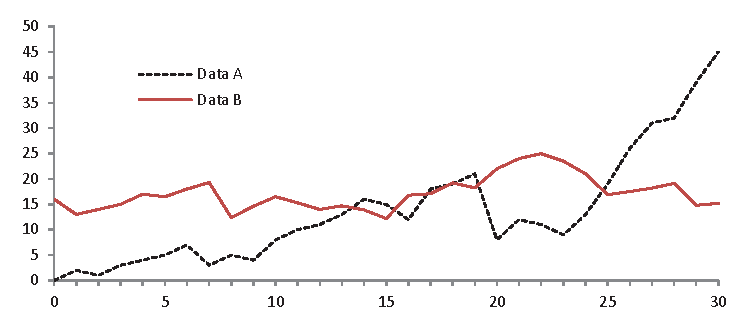
\includegraphics[width=\textwidth]{fig1.eps}
%%%justified by the macro package automatically.} 
\label{fig1}
\end{figure}

\begin{theorem}
This is a sample theorem. The run-in heading is set in bold, while
the following text appears in italics. Definitions, lemmas,
propositions, and corollaries are styled the same way.
\end{theorem}
%
% the environments 'definition', 'lemma', 'proposition', 'corollary',
% 'remark', and 'example' are defined in the LLNCS documentclass as well.
%
\begin{proof}
Proofs, examples, and remarks have the initial word in italics,
while the following text appears in normal font.
\end{proof}

%
% ---- Bibliography ----
%
% BibTeX users should specify bibliography style 'splncs04'.
% References will then be sorted and formatted in the correct style.
%
\bibliographystyle{splncs04}
\bibliography{the}
%
%
\end{document}
